%\VignetteIndexEntry{Getting started with the package}
%\VignetteKeywords{getting started}
%\VignettePackage{surveillance}

\documentclass[a4paper,11pt]{article}
\usepackage{natbib}
\bibliographystyle{apalike}

% Preabmle parts
\usepackage[T1]{fontenc}        % Make it possible to use danish characters !!
\usepackage{url}
\usepackage{hyperref}
\usepackage{times}  
\renewcommand{\sfdefault}{ptm} % Brug times som font - vigtigt i
                               % pdflatex?

%PSTricks
\usepackage{pdftricks}
\begin{psinputs}
  \usepackage{pst-all}
\end{psinputs}

\usepackage{bm}
\usepackage{amsmath}
\usepackage{amssymb}
\usepackage{latexsym}
\usepackage{verbatim}
\usepackage{epsfig}
\usepackage{comment}
\newcommand{\surveillance}{\texttt{surveillance}}
\usepackage{pdfpages}

\title{The R-Package 'surveillance'}
\author{
Michael H{\"o}hle\thanks{Author of correspondance: Department of Statistics, University of Munich, Ludwigstr.\ 33, 80539 M{\"u}nchen, Germany, Email: \texttt{hoehle@stat.uni-muenchen.de}}$\>\>$, Andrea Riebler and Michaela Paul\\
Department of Statistics\\
University of Munich\\
Germany } \date{\today}

\usepackage{d:/Programme/R/R-2.6.1/share/texmf/Sweave}
\begin{document}
%%%%%%%%%%%%%%%%%%%%%%%%%%%%%%%%%%%%%%%%%%%%%%%%%%%%%%%%%%%%%%%%%%%%%%
% Sweave 
%%%%%%%%%%%%%%%%%%%%%%%%%%%%%%%%%%%%%%%%%%%%%%%%%%%%%%%%%%%%%%%%%%%%%%
%Put all in another directory

 \setkeys{Gin}{width=1\textwidth} 

%%%%%%%%%%%%%%%%%%%%%%%%%%%%%%%%%%%%%%%%%%%%%%%%%%%%%%%%%%%%%%%%%%%%%%
% Initial R code
%%%%%%%%%%%%%%%%%%%%%%%%%%%%%%%%%%%%%%%%%%%%%%%%%%%%%%%%%%%%%%%%%%%%%%




\maketitle  
%\mbox{}\hrulefill\\

\begin{abstract}
  \noindent This document gives an introduction to the R-Package
  'surveillance' containing tools for outbreak detection in routinely
  collected surveillance data. The package contains an implementation
  of the procedures described by~\citet{stroup89},
  \citet{farrington96} and the system used at the Robert Koch
  Institute, Germany. For evaluation purposes, the package contains
  example data sets and functionality to generate surveillance data by
  simulation. To compare the algorithms, benchmark numbers like
  sensitivity, specificity, and detection delay can be computed for a
  set of time series. Being an open-source package it should be easy
  to integrate new algorithms; as an example of this process, a
  simple Bayesian surveillance algorithm is described, implemented and evaluated.\\

  \noindent{\bf Keywords:} infectious disease, monitoring, aberrations, 
  outbreak, time series of counts.
\end{abstract}


\section{Introduction}\label{sec:intro}
Public health authorities have in an attempt to meet the threats of
infectious diseases to society created comprehensive mechanisms for
the collection of disease data. As a consequence, the abundance of
data has demanded the development of automated algorithms for the
detection of abnormalities. Typically, such an algorithm monitors a
univariate time series of counts using a combination of heuristic
methods and statistical modelling.  Prominent examples of surveillance
algorithms are the work by~\citet{stroup89} and~\citet{farrington96}.
A comprehensive survey of outbreak detection methods can be found
in~\citep{farrington2003}.

The R-package \texttt{surveillance} was written with the aim of
providing a test-bench for surveillance algorithms. From the
Comprehensive R Archive Network (CRAN) the package can be downloaded
together with its source code. It allows users to test new algorithms
and compare their results with those of standard surveillance
methods. A few real world outbreak datasets are included together with
mechanisms for simulating surveillance data.  With the package at
hand, comparisons like the one described by~\citet{hutwagner2005}
should be easy to conduct.

The purpose of this document is to illustrate the basic functionality
of the package with R-code examples.  Section~\ref{sec:data} contains
a description of the data format used to store surveillance data,
mentions the built-in datasets and illustrates how to create new
datasets by simulation.  Section~\ref{sec:algo} contains a short
description of how to use the surveillance algorithms and illustrate
the results.  Further information on the individual functions can be
found in the on-line documentation of the package, which is also
provided in printed form as an Appendix of this document.

\section{Surveillance Data}\label{sec:data}
Denote by $\{y_t\>;t=1,\ldots,n\}$ the time series of counts
representing the surveillance data. Because such data typically are
collected on a weekly basis, we shall also use the alternative
notation $\{y_{i:j}\}$ with $j=\{1,\ldots,52\}$ being the week number
in year $i=\{-b,\ldots,-1,0\}$. That way the years are indexed such
that most current year has index zero. For evaluation of the outbreak
detection algorithms it is also possible for each week to store -- if
known -- whether there was an outbreak that week. The resulting
multivariate series $\{(y_t,x_t)\>; t=1,\ldots,n\}$ is in
\texttt{surveillance} given by an object of class \texttt{disProg}
(disease progress), which is basically a \texttt{list} containing two
vectors: the observed number of counts and a boolean vector
\texttt{state} indicating whether there was an outbreak that week. A
number of time series are contained in the \texttt{data} directory,
mainly originating from the SurvStat@RKI database at
\href{http://www3.rki.de/SurvStat/}{http://www3.rki.de/SurvStat/}
maintained by the Robert Koch Institute, Germany~\citep{survstat}.
For example the object \texttt{k1} describes Kryptosporidosis
surveillance data for the German federal state Baden-W�rttemberg
2001-2005. The peak in 2001 is due to an outbreak of Kryptosporidosis
among a group of army-soldiers in boot-camp~\citep{bulletin3901}. In
\surveillance\ the \texttt{readData} function is used to bring the
time series on \texttt{disProg} form. The SurvStat@RKI database at
\href{http://www3.rki.de/SurvStat/}{http://www3.rki.de/SurvStat/}
maintained by the Robert Koch Institute, Germany, uses a 53 weeks a
year format; therefore a conversion with \texttt{correct53to52} is
necessary.

\begin{Schunk}
\begin{Sinput}
> data(k1)
> plot(k1, main = "Kryptosporidiosis in BW 2001-2005")
\end{Sinput}
\end{Schunk}
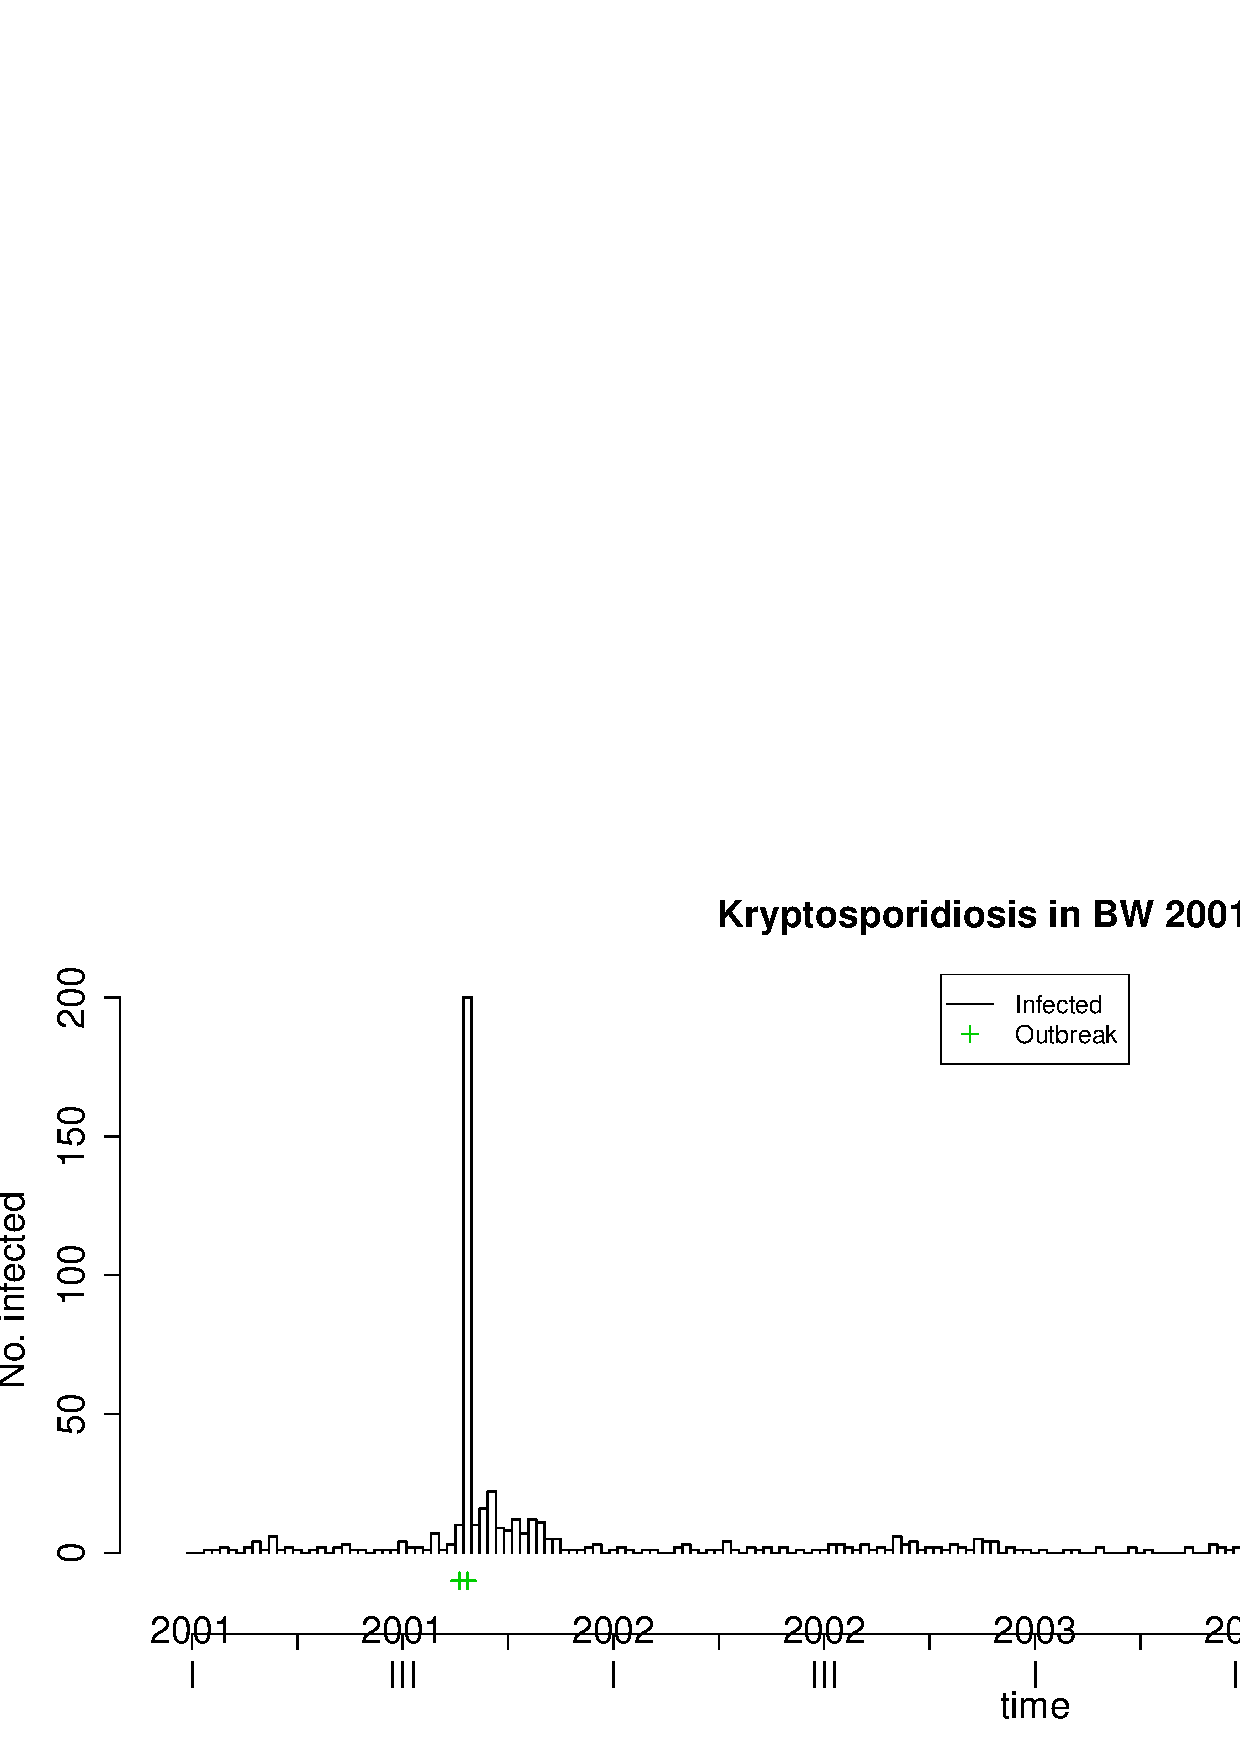
\includegraphics{figs/vignette-002}

For evaluation purposes it is also of interest to generate
surveillance data using simulation. The package contains functionality
to generate surveillance data containing point-source like outbreaks,
for example with a Salmonella serovar. The model is a Hidden Markov
Model (HMM) where a binary state $X_t, t=1,\ldots,n$, denotes whether
there was an outbreak and $Y_t$ is the number of observed
counts, see Fig.~\ref{fig:hmm}.

\begin{figure}[htbp]
  \centering
  \begin{pdfpic}
    \input pst-eps
    \TeXtoEPS
    \SpecialCoor
  \begin{pspicture}(0,0)(10,3) %lower y -2.5 would be better
   %\psgrid
   \psset{arrowsize=7pt,arrowinset=0}

   \rput(1,2.5){\ovalnode{X1}{$X_1$}}
   \rput(3,2.5){\ovalnode{X2}{$X_2$}}
   \rput(5,2.5){\ovalnode{X3}{$X_3$}}
   \rput(6.5,2.5){\ovalnode[linestyle=none]{Xinv1}{}}
   \rput(7,2.5){$\ldots$}
   \rput(7.5,2.5){\ovalnode[linestyle=none]{Xinv2}{}}
   \rput(9,2.5){\ovalnode{Xn}{$X_n$}}


   \rput(1,0.5){\ovalnode{Y1}{$Y_1$}}
   \rput(3,0.5){\ovalnode{Y2}{$Y_2$}}
   \rput(5,0.5){\ovalnode{Y3}{$Y_3$}}
   \rput(9,0.5){\ovalnode{Yn}{$Y_n$}}

   \ncline{->}{X1}{X2}
   \ncline{->}{X2}{X3}
   \ncline{->}{X3}{Xinv1}
   \ncline{->}{Xinv2}{Xn}

   \ncline{->}{X1}{Y1}
   \ncline{->}{X2}{Y2}
   \ncline{->}{X3}{Y3}
   \ncline{->}{Xn}{Yn}
 \end{pspicture}
 \endTeXtoEPS
\end{pdfpic}
\caption{The Hidden Markov Model}
  \label{fig:hmm}
\end{figure}
The state $X_t$ is a homogenous Markov chain with the following
transition matrix
\begin{center}
  \begin{tabular}{c|cc}
  $X_t\backslash X_{t+1}$ &  0      & 1\\
  \hline              $0$ & $p$     & $1 - p$ \\
                      $1$ & $1 - r$ & $r$
  \end{tabular}
\end{center}
Hence $1-p$ is the probability to switch to an outbreak state and
$1-r$ is the probability that $X_t=1$ is followed by $X_{t+1}=1$.
Furthermore, the observation $Y_t$ is Poisson-distributed with
log-link mean depending on a seasonal effect and time trend, i.e.\
\[
\log \mu_t = A \cdot \sin \, (\omega \cdot (t + \varphi)) + \alpha +
\beta t.
\]
In case of an outbreak $(X_t=1)$ the mean increases with a value of
$K$, altogether  
\begin{equation}\label{eq:hmm}
  Y_t \sim \operatorname{Po}(\mu_t + K \cdot X_t). 
\end{equation}
The model in (\ref{eq:hmm}) corresponds to a single-source,
common-vehicle outbreak, where the length of an outbreak is controlled
by the transition probability $r$. The daily numbers of outbreak-cases
are simply independently Poisson distributed with mean $K$. A
physiologically better motivated alternative could be to operate with
a stochastic incubation time (e.g.\ log-normal or gamma distributed)
for each individual exposed to the source, which results in a temporal
diffusion of the peak. The advantage of (\ref{eq:hmm}) is that
estimation can be done by a generalized linear model (GLM) using $X_t$
as covariate and that it allows for an easy definition of a correctly
identified outbreak: each $X_t=1$ has to be identified. More advanced
setups would require more involved definitions of an outbreak, e.g.\ 
as a connected series of time instances, where the number of outbreak
cases is greater than zero.  Care is then required in defining what a
correctly identified outbreak for time-wise overlapping outbreaks means.

In \surveillance\ the function \verb+sim.pointSource+ is used to
simulate such a point-source epidemic; the result is an object of class
\verb+disProg+.

\label{ex:sts}
\begin{Schunk}
\begin{Sinput}
> sts <- sim.pointSource(p = 0.99, r = 0.5, length = 400, 
+     A = 1, alpha = 1, beta = 0, phi = 0, frequency = 1, 
+     state = NULL, K = 1.7)
> plot(sts)
\end{Sinput}
\end{Schunk}
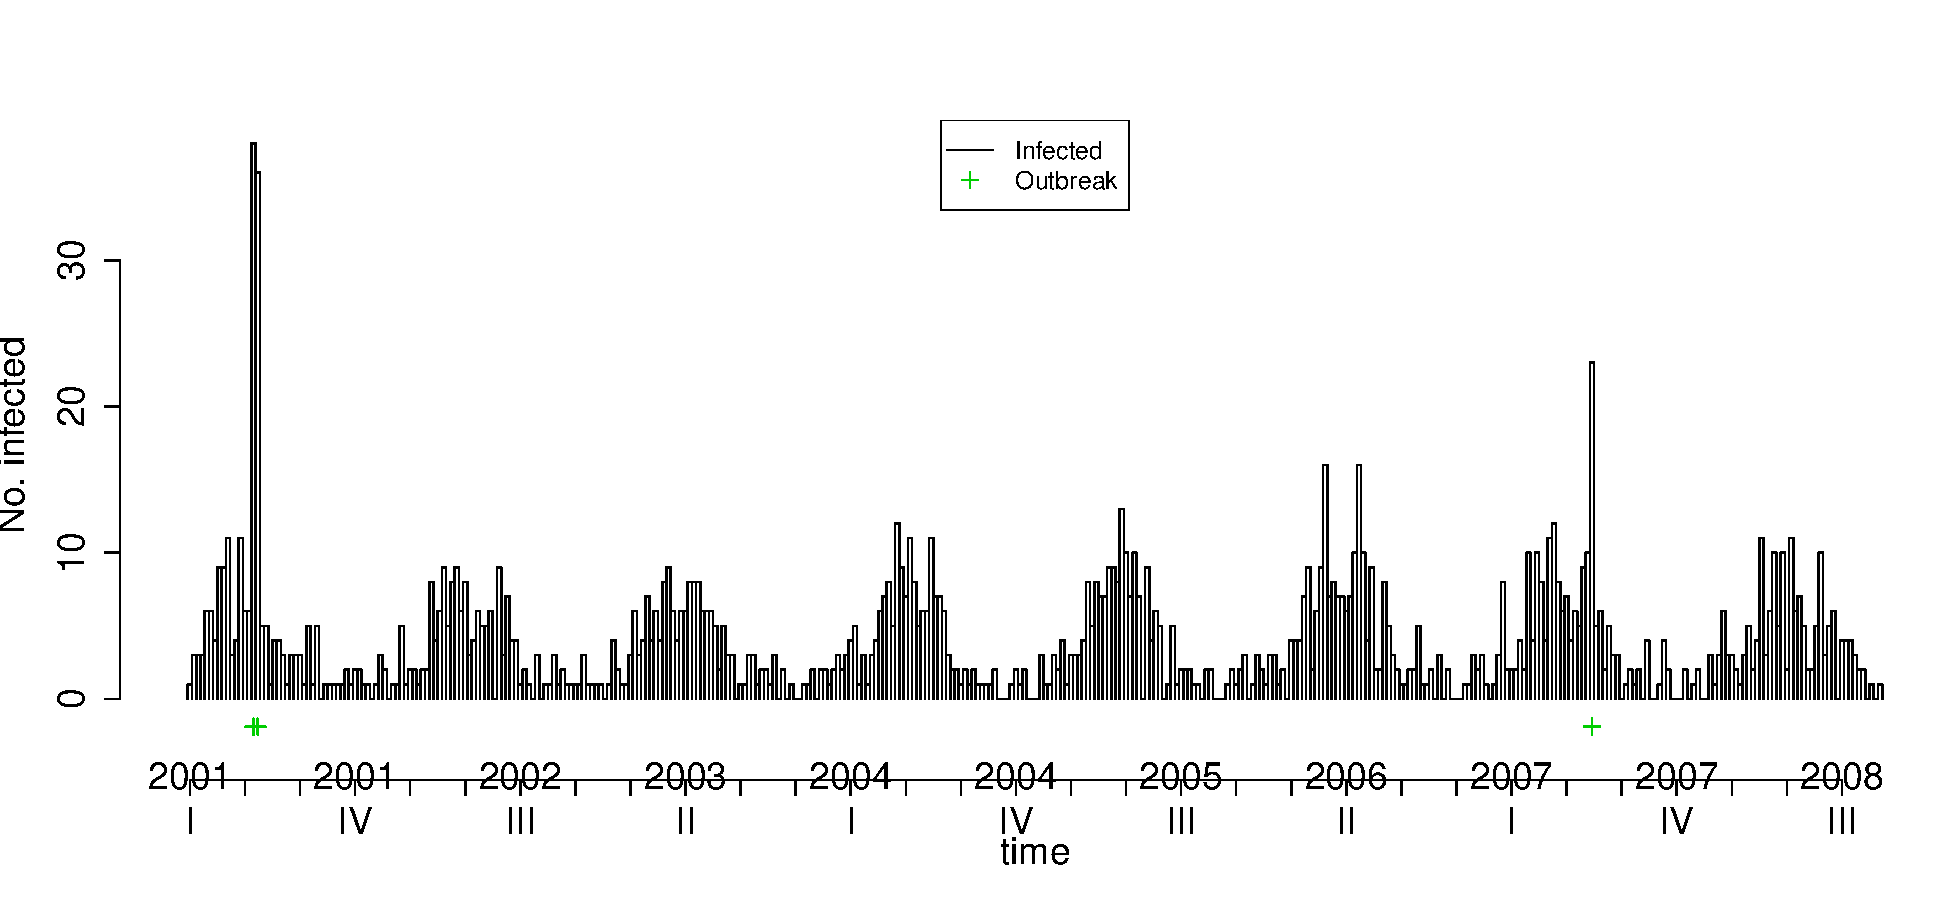
\includegraphics{figs/vignette-003}

\section{Surveillance Algorithms}\label{sec:algo}
Surveillance data often exhibit strong seasonality, therefore most
surveillance algorithms only use a set of so called \emph{reference
  values} as basis for drawing conclusions. Let $y_{0:t}$ be the
number of cases of the current week (denoted week $t$ in year $0$), $b$
the number of years to go back in time and $w$ the number of weeks
around $t$ to include from those previous years. For the year zero we
use $w_0$ as the number of previous weeks to include -- typically
$w_0=w$. Altogether the set of reference values is thus defined to be
\[
R(w,w_0,b) =
\left(\bigcup\limits_{i=1}^b\bigcup\limits_{j=\,-w}^w
  y_{-i:t+j}\right)   \cup
\left(\bigcup_{k=-w_0}^{-1} y_{0:t+k}\right)
\]
Note that the number of cases of the current week is not part of
$R(w,w_0,b)$.

A surveillance algorithm is a procedure using the reference values
to create a prediction $\hat{y}_{0:t}$ for the current week.  This
prediction is then compared with the observed $y_{0:t}$: if the
observed number of cases is much higher than the predicted number, the
current week is flagged for further investigations. In order to do
surveillance for time $0:t$ an important concern is the choice of $b$
and $w$. Values as far back as time $-b:t-w$ contribute to
$R(w,w_0,b)$ and thus have to exist in the observed time series.

Currently, we have implemented four different type of algorithms in
\surveillance.  The Centers for Disease Control and Prevention (CDC)
method~\citep{stroup89}, the Communicable Disease Surveillance Centre
(CDSC) method~\citep{farrington96}, the method used at the Robert Koch
Institute (RKI), Germany~\citep{altmann2003}, and a Bayesian approach
documented in~\citet{riebler2004}. A detailed description of each
method is beyond the scope of this note, but to give an idea of the
framework the Bayesian approach developed in~\citet{riebler2004} is
presented: Within a Bayesian framework, quantiles of the predictive
posterior distribution are used as a measure for defining alarm
thresholds.

The model assumes that the reference values are identically and
independently Poisson distributed with parameter $\lambda$ and a
Gamma-distribution is used as Prior distribution for $\lambda$.  The
reference values are defined to be $R_{\text{Bayes}}= R(w,w_0,b) =
\{y_1, \ldots, y_{n}\}$ and $y_{0:t}$ is the value we are trying to
predict. Thus, $\lambda \sim \text{Ga}(\alpha, \beta)$ and
$y_i|\lambda \sim \text{Po}(\lambda)$, $i = 1,\ldots,{n}$. Standard
derivations show that the posterior distribution is
\begin{equation*}
\lambda|y_1, \ldots, y_{n} \sim \text{Ga}(\alpha + \sum_{i=1}^{n} y_i, 
\beta + n). 
\end{equation*}
Computing the predictive distribution
\begin{equation*}
f(y_{0:t}|y_1,\ldots,y_{n}) =
\int\limits^\infty_0{f(y_{0:t}|\lambda)\,
f(\lambda|y_1,\ldots,y_{n})}\, d\lambda
\end{equation*}
we get the Poisson-Gamma-distribution
\begin{equation*}
 y_{0:t}|y_1,\ldots,y_{n} \sim 
\text{PoGa}(\alpha + \sum_{i=1}^{n} y_i, \beta + n),
\end{equation*}
which is a generalization of the negative Binomial distribution,
i.e.\ 
\[
y_{0:t}|y_1,\ldots,y_{n} \sim \text{NegBin}(\alpha + \sum_{i=1}^{n}
y_i, \tfrac{\beta + n}{\beta + n + 1}).
\]
Using the Jeffrey's Prior $\text{Ga}(\tfrac{1}{2}, 0)$ as
non-informative Prior distribution for $\lambda$ the parameters of the
negative Binomial distribution are
\begin{align*}
  \alpha + \sum_{i=1}^{n} y_i &= \frac{1}{2} + \sum_{y_{i:j} \in R_{\text{Bayes}}}\!\! y_{i:j} \quad
%  \intertext{and}
  \quad\text{and}\quad
  \frac{\beta + n}{\beta + n + 1} = \frac{|R_{\text{Bayes}}|}{|R_{\text{Bayes}}| + 1}.
\end{align*}
Using a quantile-parameter $\alpha$, the smallest value $y_\alpha$ is computed, so that
\begin{equation*}
  P(y \leq y_\alpha) \geq 1-\alpha.
\end{equation*}
Now 
\begin{equation*}
         A_{0:t} = I(y_{0:t} \geq y_\alpha),
\end{equation*}
i.e. if $y_{0:t}\geq y_\alpha$ the current week is flagged as an
alarm. As an example, the \verb+Bayes1+ method uses the last six weeks
as reference values, i.e.\ $R(w,w_0,b)=(6,6,0)$, and is applied to the
\texttt{k1} dataset with $\alpha=0.01$ as follows.

\begin{Schunk}
\begin{Sinput}
> k1.b660 <- algo.bayes(k1, control = list(range = 27:192, 
+     b = 0, w = 6, alpha = 0.01))
> plot(k1.b660, disease = "k1", firstweek = 1, startyear = 2001)
\end{Sinput}
\end{Schunk}
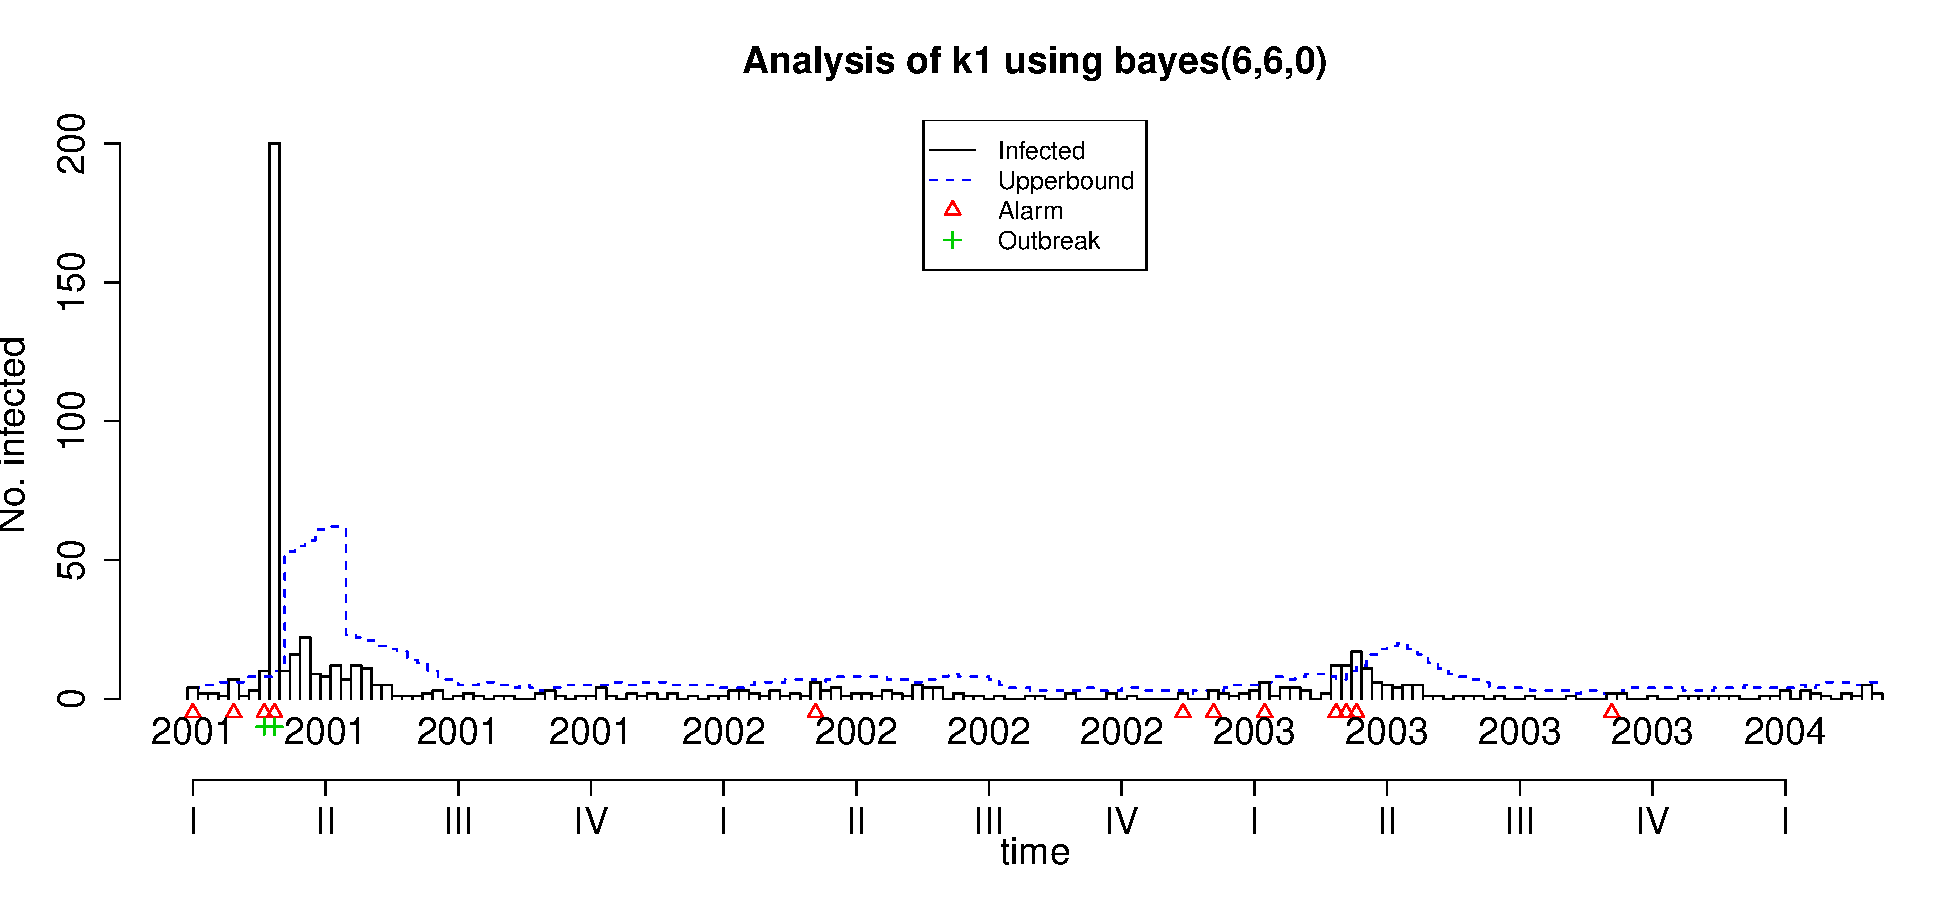
\includegraphics{figs/vignette-004}

Several extensions of this simple Bayesian approach are imaginable,
for example the inane over-dispersion of the data could be modeled by
using a negative-binomial distribution, time trends and mechanisms to
correct for past outbreaks could be integrated, but all at the cost of
non-standard inference for the predictive distribution. Here
simulation based methods like Markov Chain Monte Carlo or heuristic
approximations have to be used to obtain the required alarm
thresholds.

In general, the \verb+surveillance+ package makes it easy to add
additional algorithms -- also those not based on reference values --
by using the existing implementations as starting point.

The following call uses the CDC and Farrington procedure on the
simulated time series \verb+sts+ from page~\pageref{ex:sts}. Note that
the CDC procedure operates with four-week aggregated data -- to better
compare the upper bound value, the aggregated number of counts for
each week are shown as circles in the plot.

\begin{Schunk}
\begin{Sinput}
> cntrl <- list(range = 300:400, m = 1, w = 3, b = 5, alpha = 0.01)
> sts.cdc <- algo.cdc(sts, control = cntrl)
> sts.farrington <- algo.farrington(sts, control = cntrl)
\end{Sinput}
\end{Schunk}


\begin{Schunk}
\begin{Sinput}
> par(mfcol = c(1, 2))
> plot(sts.cdc, legend.opts = NULL)
> plot(sts.farrington, legend.opts = NULL)
\end{Sinput}
\end{Schunk}
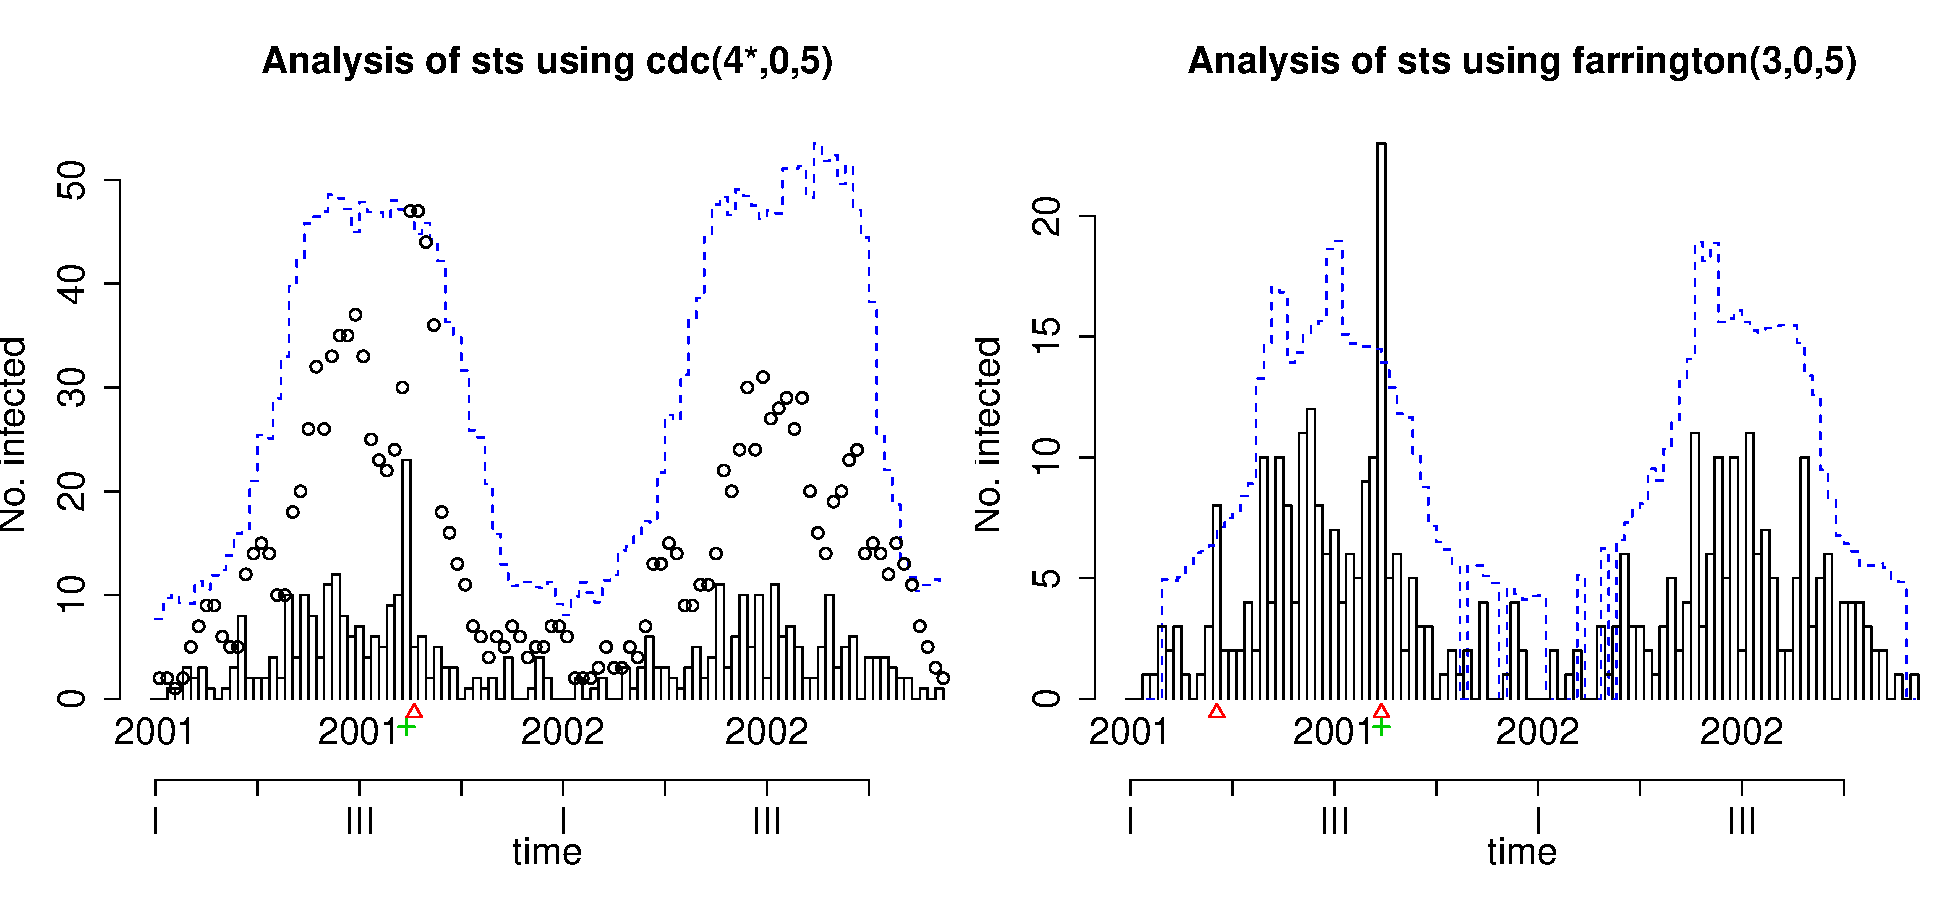
\includegraphics{figs/vignette-007}


Typically, one is interested in evaluating the performance of the
various surveillance algorithms. An easy way is to look at the
sensitivity and specificity of the procedure -- a correct
identification of an outbreak is defined as follows: if the algorithm
raises an alarm for time $t$, i.e.\ $A_t=1$ and $X_t=1$ we have a
correct classification, if $A_t=1$ and $X_t=0$ we have a
false-positive, etc. In case of more involved outbreak models, where
an outbreak lasts for more than one week, a correct identification
could be if at least one of the outbreak weeks is correctly
identified, see e.g.\ \citet{hutwagner2005}.

To compute various performance scores the function
\verb+algo.quality+ can be used on a \verb+SurvRes+ object.

\begin{Schunk}
\begin{Sinput}
> print(algo.quality(k1.b660))
\end{Sinput}
\begin{Soutput}
     TP FP TN  FN Sens Spec      dist       mlag
[1,] 2  10 154 0  1    0.9390244 0.06097561 0   
\end{Soutput}
\end{Schunk}
This computes the number of false positives, true negatives, false
negatives, the sensitivity and the specificity. Furthermore, \texttt{dist}
is defined as
\[
\sqrt{(Spec-1)^2 + (Sens - 1)^2},
\]
that is the distance to the optimal point $(1,1)$, which serves as a
heuristic way of combining sensitivity and specificity into a single
score. Of course, weighted versions are also imaginable.  Finally,
\texttt{lag} is the average number of weeks between the first of a
consecutive number of $X_t=1$'s (i.e.\ an outbreak) and the first
alarm raised by the algorithm.

To compare the results of several algorithms on a single time series
we declare a list of control objects -- each containing the name and
settings of the algorithm we want to apply to the data.
\begin{Schunk}
\begin{Sinput}
> control = list(list(funcName = "rki1"), list(funcName = "rki2"), 
+     list(funcName = "rki3"), list(funcName = "bayes1"), 
+     list(funcName = "bayes2"), list(funcName = "bayes3"), 
+     list(funcName = "cdc", alpha = 0.05), list(funcName = "farrington", 
+         alpha = 0.05))
> control <- lapply(control, function(ctrl) {
+     ctrl$range <- 300:400
+     return(ctrl)
+ })
\end{Sinput}
\end{Schunk}
%
In the above, \texttt{rki1}, \texttt{rki2} and \texttt{rki3} are three
methods with reference values $R_\text{rki1}(6,6,0)$,
$R_\text{rki2}(6,6,1)$ and $R_\text{rki3}(4,0,2)$ all called with
$\alpha=0.05$. The methods \texttt{bayes1}-\texttt{bayes3} is the
Bayesian algorithm using the same setup of reference values. The CDC
Method is special, since it operates on aggregated four-week blocks.
To make everything comparable a common $\alpha=0.05$ level is used for
all algorithms. All algorithms in \texttt{control} are applied to
\texttt{sts} using:
\begin{Schunk}
\begin{Sinput}
> algo.compare(algo.call(sts, control = control))
\end{Sinput}
\end{Schunk}
\begin{Schunk}
\begin{Soutput}
                  TP FP TN FN sens spec dist mlag
rki(6,6,0)        1  6  94 0  1    0.94 0.06 0   
rki(6,6,1)        1  1  99 0  1    0.99 0.01 0   
rki(4,0,2)        1  1  99 0  1    0.99 0.01 0   
bayes(6,6,0)      1  14 86 0  1    0.86 0.14 0   
bayes(6,6,1)      1  8  92 0  1    0.92 0.08 0   
bayes(4,0,2)      1  5  95 0  1    0.95 0.05 0   
cdc(4*,0,5)       1  4  96 0  1    0.96 0.04 0   
farrington(3,0,5) 1  3  97 0  1    0.97 0.03 0   
\end{Soutput}
\end{Schunk}
%res <- algo.compare(algo.call(sts,control=control))
%xtable(res,digits=c(0,0,0,0,0,2,2,2,2))


A test on a set of time series can be done as follows. Firstly, a list
containing 10 simulated time series is created. Secondly, all the
algorithms specified in the \texttt{control} object are applied to
each series. Finally the results for the 10 series are combined in one
result matrix.

\begin{Schunk}
\begin{Sinput}
> ten <- lapply(1:10, function(x) {
+     sim.pointSource(p = 0.975, r = 0.5, length = 400, 
+         A = 1, alpha = 1, beta = 0, phi = 0, frequency = 1, 
+         state = NULL, K = 1.7)
+ })
\end{Sinput}
\end{Schunk}
\begin{Schunk}
\begin{Sinput}
> ten.surv <- lapply(ten, function(ts) {
+     algo.compare(algo.call(ts, control = control))
+ })
\end{Sinput}
\end{Schunk}
\begin{Schunk}
\begin{Sinput}
> algo.summary(ten.surv)
\end{Sinput}
\end{Schunk}
\begin{Schunk}
\begin{Soutput}
                  TP FP  TN FN sens spec dist mlag
rki(6,6,0)        32 23 940 15 0.68 0.98 0.32 4.27
rki(6,6,1)        34  5 958 13 0.72 0.99 0.28 2.93
rki(4,0,2)        35  4 959 12 0.74 1.00 0.26 1.98
bayes(6,6,0)      40 90 873  7 0.85 0.91 0.18 1.32
bayes(6,6,1)      41 53 910  6 0.87 0.94 0.14 0.72
bayes(4,0,2)      45 42 921  2 0.96 0.96 0.06 0.00
cdc(4*,0,5)       21 34 929 26 0.45 0.96 0.55 8.05
farrington(3,0,5) 36 14 949 11 0.77 0.99 0.23 2.65
\end{Soutput}
\end{Schunk}
%xtable(algo.summary(ten.surv),digits=c(0,0,0,0,0,2,2,2,2))

A similar procedure can be applied when evaluating the 14 surveillance
series drawn from SurvStat@RKI~\citep{survstat}. A problem is however,
that the series after conversion to 52 weeks/year are of length 209 weeks.
This is insufficient to apply e.g.\ the CDC algorithm. To conduct the
comparison on as large a dataset as possible the following trick is
used: The function \texttt{enlargeData} replicates the requested
\texttt{range} and inserts it before the original data, after which
the evaluation can be done on all 209 values.

\begin{Schunk}
\begin{Sinput}
> range = (2 * 4 * 52) + 1:length(k1$observed)
> control <- lapply(control, function(cntrl) {
+     cntrl$range = range
+     return(cntrl)
+ })
> outbrks <- c("m1", "m2", "m3", "m4", "m5", "q1_nrwh", 
+     "q2", "s1", "s2", "s3", "k1", "n1", "n2", "h1_nrwrp")
> outbrks <- lapply(outbrks, function(name) {
+     eval(substitute(data(name), list(name = name)))
+     enlargeData(get(name), range = 1:(4 * 52), times = 2)
+ })
> one.survstat.surv <- function(outbrk) {
+     algo.compare(algo.call(outbrk, control = control))
+ }
\end{Sinput}
\end{Schunk}
\begin{Schunk}
\begin{Sinput}
> algo.summary(lapply(outbrks, one.survstat.surv))
\end{Sinput}
\end{Schunk}
\begin{Schunk}
\begin{Soutput}
                   TP  FP   TN  FN  sens  spec  dist mlag
rki(6,6,0)         38  62 2646 180 0.174 0.977 0.826 5.43
rki(6,6,1)         65  83 2625 153 0.298 0.969 0.703 5.57
rki(4,0,2)         80 106 2602 138 0.367 0.961 0.634 5.43
bayes(6,6,0)       61 206 2502 157 0.280 0.924 0.724 1.71
bayes(6,6,1)      123 968 1740  95 0.564 0.643 0.564 1.36
bayes(4,0,2)      162 920 1788  56 0.743 0.660 0.426 1.36
cdc(4*,0,5)        65  94 2614 153 0.298 0.965 0.703 7.14
farrington(3,0,5)  43  71 2637 175 0.197 0.974 0.803 4.79
\end{Soutput}
\end{Schunk}

In both this study and the earlier simulation study the Bayesian
approach seems to do quite well. However, the extent of the
comparisons do not make allowance for any more supported statements.
Consult the work of~\citet{riebler2004} for a more thorough
comparision using simulation studies.

\section{Multivariate surveillance}

As of version 0.9-2 \surveillance\ supports the visualization of
multivariate time series of counts. An (multivariate) object of class
\texttt{disProg} contains matrices with the observed number of counts
and the respective state chains, where each column represents an
individual time series.  Additional elements of the
\texttt{disProg}-object are a neighbourhood matrix and a matrix with
population counts. However, only modelling of the time series as
by~\citet{held2005} is currently available. In the near future the
surveillance algorithms will also be extended to handle these
multivariate data.

For example, consider the weekly counts of new measles cases for each
``Kreis'' (area) of the administrative district ``Weser-Ems'' in Lower
Saxony, Germany, in 2001 and
2002~\citep{survstat}. Figure~\ref{fig:map} shows a map of the $m=15$
areas.  The corresponding $m \times m$ neighbourhood matrix has
elements 1 if two areas share a common border and is 0 otherwise.

\begin{figure}[htb]
  \centering
  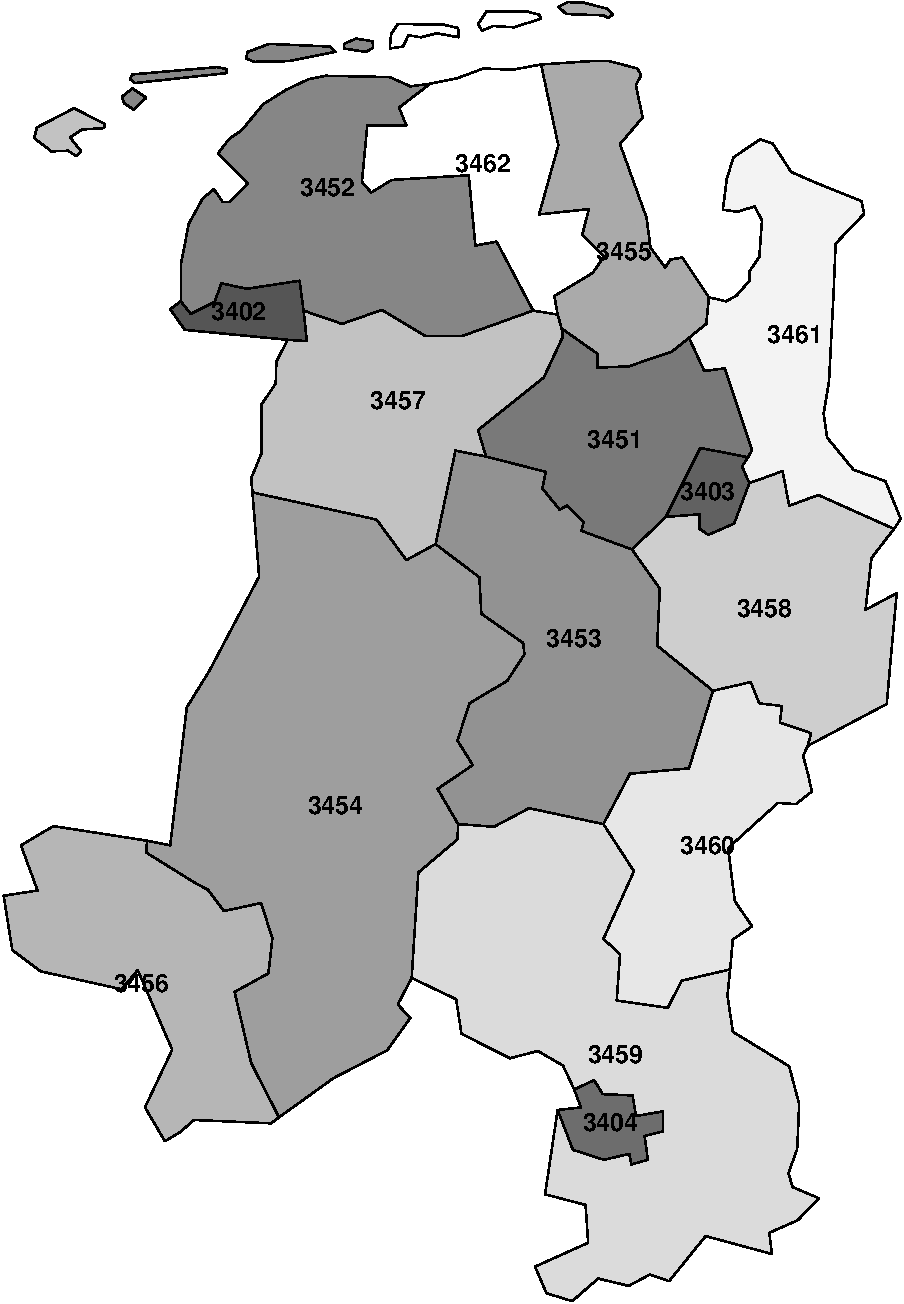
\includegraphics[width=0.5\textwidth]{figs/weseremsmap2}
  \caption{Map of the administrative district ``Weser-Ems''}     
  \label{fig:map}
\end{figure}

In the package \texttt{surveillance} the measles data are already available
in the form of a \texttt{disProg}-object.

\begin{Schunk}
\begin{Sinput}
> data(measles.weser)
> plot(measles.weser, title = "measles in Weser-Ems 2001-2002", 
+     xaxis.years = TRUE, startyear = 2001, firstweek = 1)
\end{Sinput}
\end{Schunk}
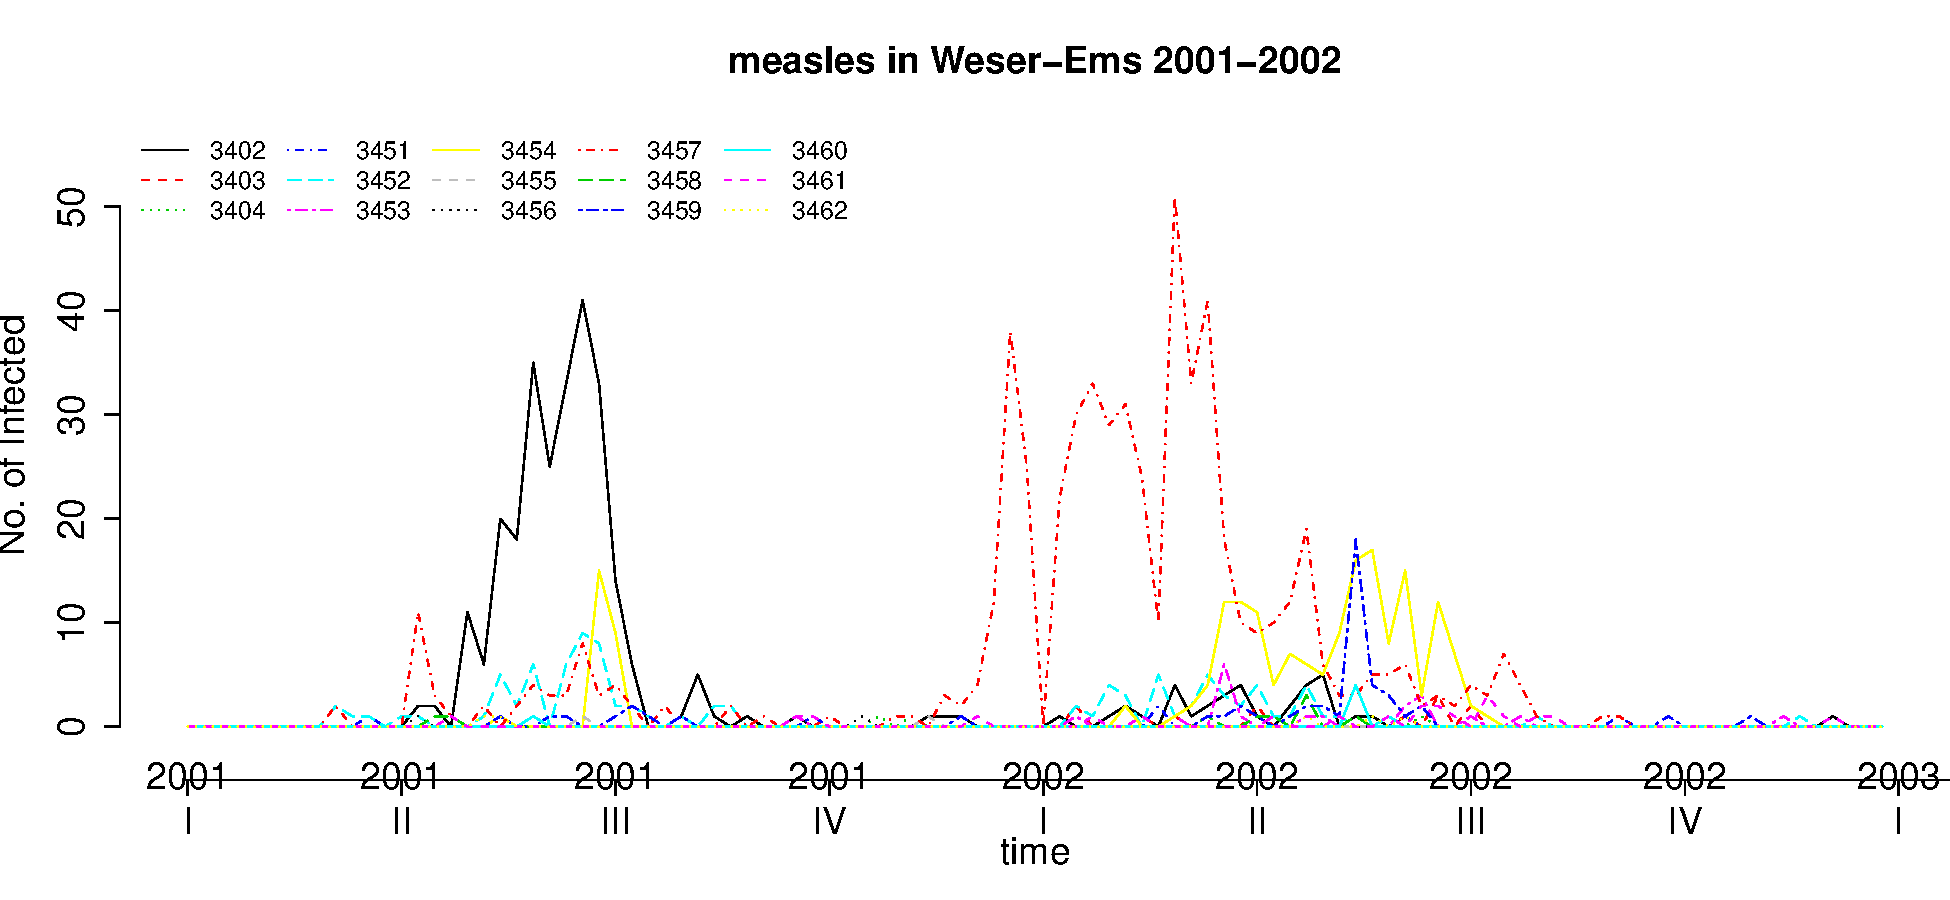
\includegraphics{figs/vignette-020}

The number of counts for each area can also be looked at and plotted
as individual time series.
Here, the x-axis is the week number since 1st of January 2001 and the 
y-axis is the number of measles cases.

\begin{Schunk}
\begin{Sinput}
> plot(measles.weser, as.one = FALSE, xaxis.years = FALSE)
\end{Sinput}
\end{Schunk}
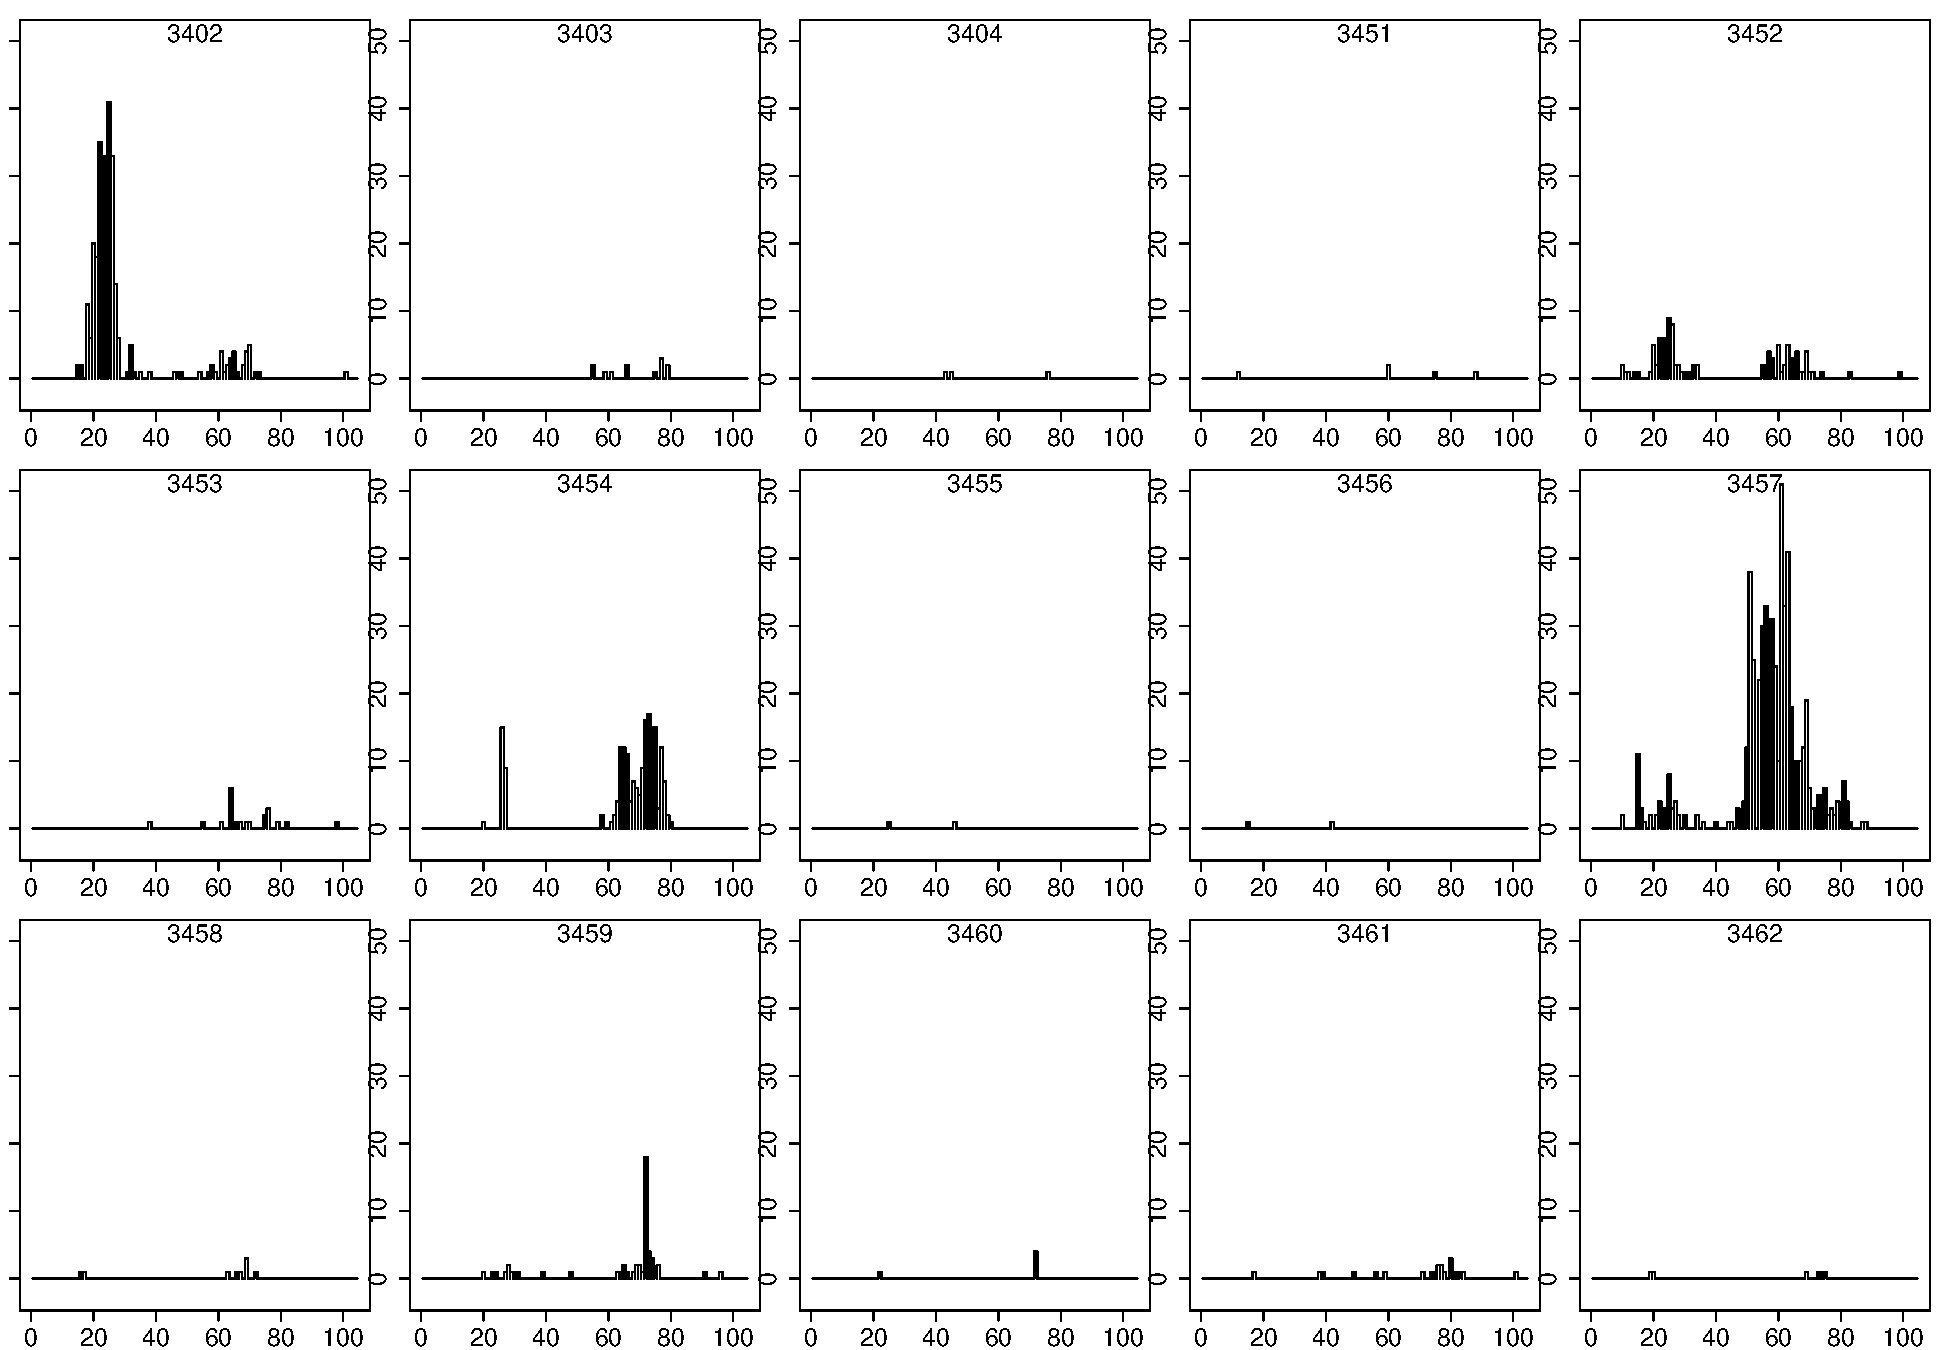
\includegraphics{figs/vignette-021}
\vspace{1em}

The data are analysed using the model proposed by \citet{held2005}.
A call to the function \texttt{algo.hhh} fits a Poisson or negative binomial
model with mean
\[
  \mu_{it} = \lambda y_{i,t-1} + \phi \sum_{j \sim i} y_{j,t-1} + n_{it} \nu_{it}\, , \quad
  i=1,\ldots,m, \, t=1,\ldots,n \, ,
\]
where $j \sim i$ denotes all neighbours of $i$,
to a multivariate time series of counts.
It is estimated  by maximum likelihood using numerical optimization methods.
The $n_{it}$ are standardized population counts and
$\log \nu_{it} = \alpha_i + \beta t + \sum_{s=1}^{S}\big(\gamma_s sin(\omega_s t)
+ \delta_s cos(\omega_s t)\big)$ with Fourier frequencies $\omega_s$.


For the weekly measles data $\omega_s=2s\pi/52$ (i.e.\ \texttt{period}=52).
In the following, the model specified in \texttt{cntrl}
is fitted to the data. The counts are assumed to be negative binomial distributed
with mean $\mu_{it}$ and variance $\mu_{it} +\mu_{it}^2/\psi$.
A linear time trend $\beta$, seasonal parameters $\gamma_1$ and $\beta_1$ (i.e.\ $S=1$)
as well as the autoregressive parameters $\lambda$ and $\phi$ are included
to specify the mean.
All in all, there are %21 parameters to be estimated.
$2S+m+4$ parameters to be estimated for the negative binomial model. 
In case of a Poisson model, the number of parameters reduces by one 
as the overdispersion parameter $\psi$ is omitted.

\begin{Schunk}
\begin{Sinput}
> cntrl <- list(linear = TRUE, season = list(nseason = 1), 
+     neighbours = TRUE, negbin = "single", lambda = TRUE)
> measles.hhh <- algo.hhh(measles.weser, control = cntrl)
\end{Sinput}
\end{Schunk}

Depending on the inital values for the parameters, the optimization algorithm
might not converge or only find a local maximum as the parameter space is
high-dimensional.
It is therefore reasonable to try multiple starting values.

The function \texttt{create.grid} takes a \texttt{list} with elements in the
form of \texttt{param = c(lower,upper,length)} to create a matrix of starting
values.
For each parameter a sequence of length \texttt{length} from \texttt{lower}
to \texttt{upper} is built and the resulting grid contains all
combinations of these parameter values.
A call to \texttt{algo.hhh.grid} conducts a grid search
until either all starting values are used or a time limit \texttt{maxTime} (in seconds)
is exceeded. The result with the highest likelihood is returned.

%algo.hhh.grid
\begin{Schunk}
\begin{Sinput}
> cntrl <- list(linear = TRUE, season = list(nseason = 1), 
+     neighbours = TRUE, negbin = "single", lambda = TRUE)
> grid <- create.grid(measles.weser, cntrl, params = list(endemic = c(lower = -0.5, 
+     upper = 0.5, length = 3), epidemic = c(0.1, 0.9, 
+     5), negbin = c(0.3, 12, 5)))
> algo.hhh.grid(measles.weser, control = cntrl, thetastartMatrix = grid, 
+     maxTime = 900)
\end{Sinput}
\end{Schunk}
\begin{Schunk}
\begin{Soutput}
size of grid:  375 
convergences:  60 
time needed (in seconds) 130.99 

values of log-likelihood:
-910 
  60 

Estimated parameters and standard errors: 

                  Estimates  Std.Error
3402                  2.048      0.335
3403                 -0.481      0.411
3404                 -1.914      0.652
3451                 -1.216      0.708
3452                  0.742      0.339
3453                 -0.197      0.448
3454                  0.071      0.332
3455                 -2.165      1.274
3456                 -2.101      0.766
3457                  2.254      0.277
3458                 -0.812      0.482
3459                 -0.596      0.374
3460                 -1.263      0.542
3461                  0.315      0.391
3462                 -0.662      0.612
lambda                0.498      0.074
phi                   0.001      0.003
t                     0.012      0.004
A(2 * pi * t/52)      1.447      0.163
s(2 * pi * t/52)     -0.419      0.089
psi                   0.575      0.075

log-likelihood:	 -910.3 
AIC:		 1862.5 
\end{Soutput}
\end{Schunk}



\section{Discussion and Future work}
Many extensions and additions are imaginable to improve the package.
For now, the package is intended as an academic tool providing a
test-bench for integrating new surveillance algorithms. Because all
algorithms are implemented in R, performance has not been an issue.
Especially the current implementation of the Farrington Procedure is
rather slow and would benefit from an optimization possible with
fragments written in C.

One important improvement would be to provide more involved mechanisms
for the simulation of epidemics. In particular it would be interesting
to include multi-day outbreaks originating from single-source
exposure, but with delay due to varying incubation
time~\citep{hutwagner2005} or SEIR-like
epidemics~\citep{andersson2000}. However, defining what is meant by a
correct outbreak identification, especially in the case of overlapping
outbreaks, creates new challenges which have to be met.

\section{Acknowledgements}
We are grateful to K.\ Stark and D.\ Altmann, RKI, Germany, for
discussions and information on the surveillance methods used by the
RKI. Our thanks to C.\ Lang, University of Munich, for his work on the
R--implementation and M.  Kobl, T.  Schuster and M. Rossman,
University of Munich, for their initial work on gathering the outbreak
data from SurvStat@RKI. The research was conducted with financial
support from the Collaborative Research Centre SFB 386 funded by the
German research foundation (DFG).


%\renewcommand{\bibsection}{\section{REFERENCES}}
\bibliography{references}

\end{document}
